\documentclass{report}
\usepackage{amsmath}
\usepackage{graphicx}
\usepackage{hyperref}
\newcommand{\bmathc}{\begin{center}\begin{math}}
\newcommand{\emathc}{\end{math}\end{center}}
\author{dsp@2f30.org}
\title{1D plasma simulation using the sagdeev pseudopotential approach}
\begin{document}
\maketitle
\section{Theory}
\subsection{Model}
We wish to study the propagation of ion acoustic waves propagating in an ion-electron plasma.
Starting from the continuity equation
\begin{equation} \label{Model:continuity}
\frac{\partial n}{\partial t} + \frac{\partial (n v)}{\partial x} = 0
\end{equation}
and the momentum equation
\begin{equation} \label{Model:momentum}
\frac{\partial v}{\partial t} + v \frac{\partial v}{\partial x} = - \frac{e}{m} \frac{\partial \phi}{\partial x}
\end{equation}
where $\phi$ is the electrostatic potential $m$ the mass of the ions and $e$ the charge of electrons.
Since the electron distribution has a Boltzmann density profile we have $n_e = n_0 exp(e\phi/k_B T)$ where $n_0$ the
equlibrium density $k_B$ the Boltzmann constant and $T$ the electron temperature.
Finally we have the Poisson equation
\begin{equation} \label{Model:poisson}
\epsilon_0 \frac{\partial^2 \phi}{\partial x^2} = e \left[ n_0 exp\left(\frac{e \phi}{k_B T}\right) - n \right]
\end{equation}
To move to dimensionless quantities we map
\begin{equation} \label{Model:scaling}
\begin{aligned}
	n \rightarrow n_0 \\
	\phi \rightarrow k_B T/e \\
	v \rightarrow c_{i,s} \leftarrow  c_{i,s}^2 = k_B T/m \\
	t \rightarrow \omega_{pi}^{-1} \leftarrow \omega_{pi}^{2} = \frac{n_0 e^2}{\epsilon_0 m} \\
	x \rightarrow \lambda_D \leftarrow \lambda_D^2 = \frac{\epsilon_0 k_B T}{n_0 e^2}
\end{aligned}
\end{equation}
Finally we move to our dimensionless set of equations
\begin{equation} \label{Modem:systemnodim}
\begin{aligned}
	\frac{\partial n}{\partial t} + \frac{\partial (n v)}{\partial x} = 0 \\
	\frac{\partial v}{\partial t} + v \frac{\partial v}{\partial x} = -\frac{\partial \phi}{\partial x} \\
	\frac{\partial^2 \phi}{\partial x^2} = e^{\phi} - n
\end{aligned}
\end{equation}

\subsection{Sagdeev pseudopotential}
We will consider propagating excitations that retain their shape if we follow them in a moving frame.
Performing a change of variables 
\bmathc
	X = x - M t
\emathc

\section{implementation}
\subsection{Sagdeev pseudopotential root finding}
We constructed a safe newton method {\tt NewtonSafe} to calculate the root of $S(\phi, M) = 0$
for various Mach numbers.

\begin{tabular}{c | c}
Mach & phi where S(phi, M) = 0 \\
\hline
1.04 &  0.116533567622633\\
1.05 &  0.144633267184183\\
1.08 &  0.226627117580462\\
1.09 &  0.25322342866721\\
1.1  & 0.279468030965999\\
1.11 &  0.305369862773675\\
1.12 &  0.330937533957688\\
1.13 &  0.356179341545776\\
1.14 &  0.381103284415865\\
1.15 &  0.405717077147053\\
1.16 &  0.430028163087686\\
1.17 &  0.454043726692463\\
1.18 &  0.47777070517636\\
1.19 &  0.501215799529773\\
1.2  & 0.524385484935905\\
1.22 &  0.569923459224529\\
1.23 &  0.592303655566642\\
1.24 &  0.614432275102266\\
1.25 &  0.636314801831128\\
1.26 &  0.657956545845352\\
1.28 &  0.700538099147746\\
1.3  & 0.742216200770249\\
1.31 &  0.762728077320337\\
1.32 &  0.783027756464394\\
1.33 &  0.803119512631068\\
1.34 &  0.82300749462909\\
1.35 &  0.842695730449329\\
1.37 &  0.881488498684103\\
1.38 &  0.900600523140389\\
1.39 &  0.919527793642503\\
1.4  & 0.938273798682659\\
1.41 &  0.956841930439692\\
1.42 &  0.975235488243672\\
1.43 &  0.993457681887917\\
1.44 &  1.01151163479631\\
1.45 &  1.02940038705335\\
1.46 &  1.04712689830402\\
1.5  & 1.11646706298337\\
1.54 &  1.18342901913831\\
1.55 &  1.19981655919382\\
1.56 &  1.2\\
1.57 &  1.2\\
1.58 &  1.2\\
1.59 &  1.2\\
1.6  & 1.2\\
\hline
\end{tabular}

The roots as a function of the Mach number
\begin{figure}
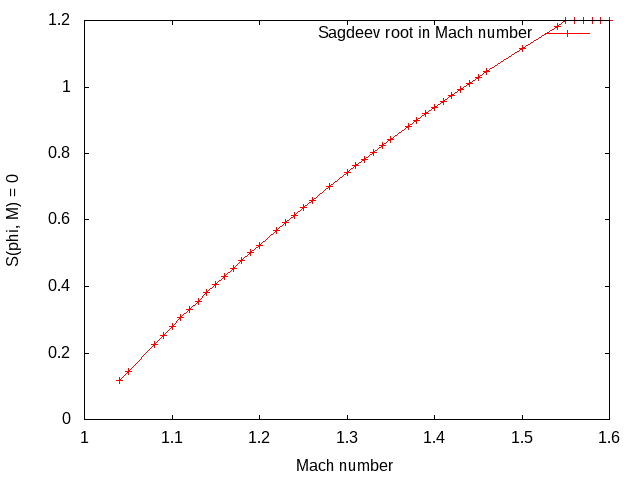
\includegraphics{sagdeevroots.png}
\end{figure}
An animation of the plot of the Sagdeev function as the Mach number changes can be viewed at 
\href{https://github.com/ramrunner/mhd-lisp/blob/master/doc/anim.gif}{my github}

\subsection{numerical construction of potential and electric fields}
We create a iterative numerical scheme to approximate $\phi$ and $E$
\begin{figure}
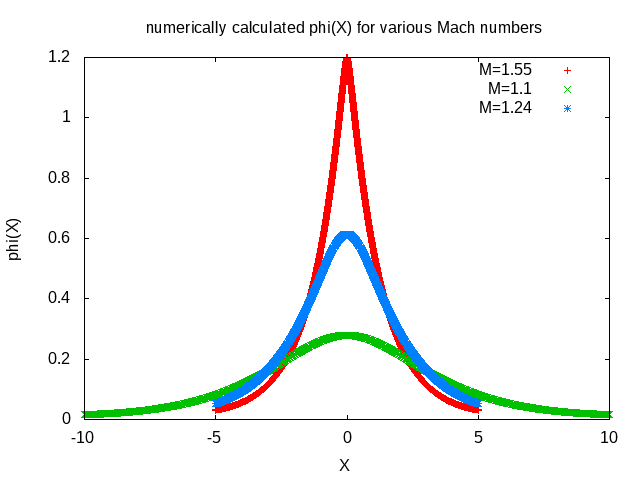
\includegraphics{phiofxvarm.png}
\end{figure}

\end{document}
